\chapter{Methods}
\section{Participants}
In the present study, we had a total population of 42 subjects, equally divided into two groups: 21 individuals were part of the healthy control group, whilst the remaining 21 were patients who suffered from a cortical or subcortical stroke. The recruitment for the control group was made through several methods: in person, talking to alumni of the \href{https://www.experiencia.ub.edu/ca/}{Universitat de l'Experiència of Barcelona}, through personal contacts, and using the platform \href{https://www.sona-systems.com/}{Sonasystem}. \\
On the other hand, to recruit participants who experienced a stroke we used a database previously employed in another study made in the \href{https://brainvitge.org/}{Cognition and Brain Plasticity Unit} for movement rehabilitation with music therapy. Furthermore, we were also able to present our study at \href{https://www.fundacioictus.com/}{Fundaciò Ictus}, where we could select more participants. \\ 
The exclusion criteria in both groups were: no visual or auditory impairments and no pregnancy.

Participants of the two groups were matched by age and gender, where we can find a mean of 55,4 years old in the control group and of 56,4 for the stroke patients, with a non-significant difference (\textit{t} test: -0.299, \textit{p} value: .766). Likewise, the difference is gender didn't result significantly different (\textit{t} test: 1.56, \textit{p} value: .127), even though a majority of men in the stroke group and a preponderance of women in the control group could be observed. \\ To both groups a questionnaire measuring the level pf physical activity was administrated: an average of 7026,78 kilojoules a day was found for the control group, whilst for the stroke group it resulted of 5669,19 kJ/d, which results lower than the control group, but still without a significant difference (\textit{t} test: 1.06, \textit{p} value: .146). \\
For what concerns the stroke group, the clinical history of the patients was collected, founding the majority of patients with the injured left hemisphere, which affected their contralateral right extremity (\textit{N=}13 suffered the injury in the left hemisphere; \textit{N=}7 in the right hemisphere; \textit{N=}1 in both hemispheres).\\ 
Participants signed an informed consent before the experiment, and they were reimbursed for their time. 
% This study was conducted according to the ethical rules presented in the General Ethical Protocol of the Faculty of Psychology and Educational Sciences.

\section{Materials}
The experiment was conducted with electroencephalography, recorded using a standard set-up with 64 Ag-AgCl electrodes placed on the scalp according to the International 10/10 system (\href{https://www.easycap.de/}{EasyCap}) to capture the neural activity in the whole brain. \\
The study presented auditory and visual stimuli related to the walking ability, all set at the frequency of 2 Hz, using Matlab for the visual stimuli and \href{https://www.audacityteam.org/}{Audacity software} for the auditory ones; resulting the best to activate neural entrainment (Matamala et al. in preparation).

For what concerns the visual stimuli, a point-light figure walking, representing the human body through white dots set in the primary joints of the body (Figure: \ref{fig: visual stimuli}), was used: it was created with \href{https://www.biomotionlab.ca/html5-bml-walker/}{BioMotionLab}, using a neutral subject, without any specific gender nor emotional display, with an average weight. After being created with the mentioned software, its frequency was adjusted to the desired one. The choice of a neutral point-light figure as the visual stimulus was made to focus only on brain activity elicited by movement processing frequency. Earlier studies have in fact shown that the presence of different important biological and social features that can be inferred from figures may enhance and grab other processes not primarily related to movement perception \parencite{Cracco_2022}. \\
For the audio stimuli, the sound of footsteps at 2 Hz with a neutral connotation was engaged (Figure: \ref{fig: audio stimuli}). The participants listened to the sound through headphones and at contemporary they were asked to watch a blue fixation cross presented in the middle of the black screen in front of them in order to keep their eyes opened. \\
Finally, a third stimulus consisting of the union of the point-light figure walking and the sounds of the footsteps, was employed and denominated as audiovisual. 
\begin{figure}[h]
    \centering
    \begin{subfigure}[h]{0.4\textwidth}
        \centering
        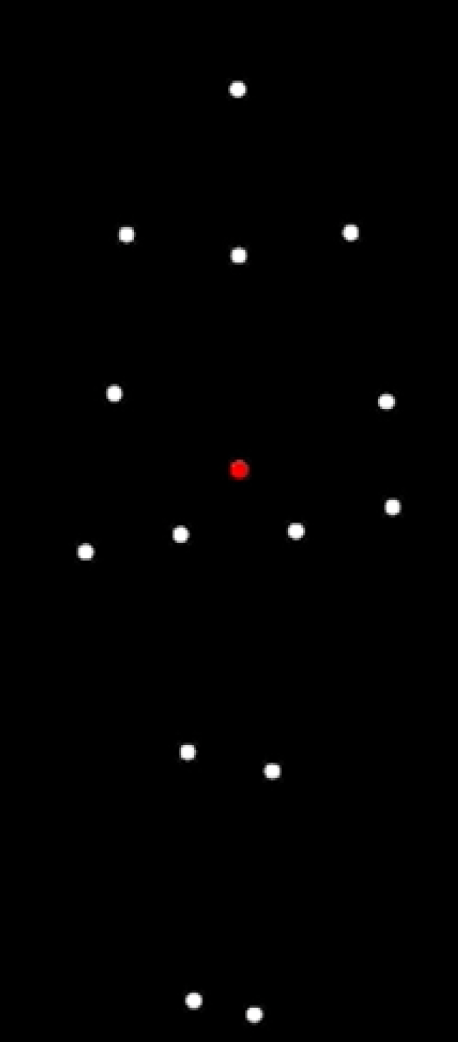
\includegraphics[width=0.35\textwidth]{appendix/point_light_figure.png}
        \caption{Point-light figure used for visual condition}
        \label{fig: visual stimuli}
    \end{subfigure}
    \hspace{4em}
    \begin{subfigure}[h]{0.4\textwidth}
        \centering
        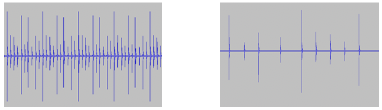
\includegraphics[width=0.85\textwidth]{appendix/audio_images.png}
        \caption{Rhythmic and random audio stimuli}
        \label{fig: audio stimuli}
    \end{subfigure}
    \label{fig: stimuli}   
\end{figure} \\
Moreover, six behavioral questions were presented (they can be found in Figure \ref{fig: Behavioral questions}): they referred to how the participant felt while seeing the point-light figure walking or listening to the footsteps sound. The questions had to be answered on a Likert scale with values between 1 (strongly disagree) to 5 (strongly agree). \\
The experiment was structured with the software \href{https://pstnet.com/products/e-prime/}{E-prime}, which allowed us to build an experiment with different stimuli presentations (e.g. adding images, questions and text).

To measure the level of physical activity of each participant, which would be later correlated to the EEG results, we used the \textit{Active-Q} questionnaire, which was created precisely to assess the total physical activity and inactivity in adults, through a series of multiple choice questions (referred to a one-year time) on daily activity, mean of transportation used, leisure and sports activities; and the time a day spent for each of them \parencite{Bonn_2012}. \\
The questionnaire was translated in Spanish from the original English version and transformed from a PDF file into an interactive digital version using the platform \href{https://www.qualtrics.com/uk/?rid=ip&prevsite=en&newsite=uk&geo=ES&geomatch=uk}{Qualtrics}. 

\section{Experimental design}
The current study is a mix models study design presenting both auditory (footstep sound) and visual (walking point-light figure) inputs at the frequency rate of 2 Hz in a rhythmic or random sequence, in three different experimental blocks: i) Auditory task, ii) Visual task and iii) Audiovisual task. The blocks were presented in a randomized order to all the participants. \\
At the beginning of our experimental session we included a text with the instructions and right afterwards a white fixation cross preceding each stimulus, which lasted five seconds and gave time to the participant to prepare themselves. 

In each experimental block the stimuli were repeated eight times: they were counterbalanced between participants being presented in a random order by their synchronicity or asynchronicity, and the number of variations used as a focus tool. These refer to the changes of the pitch (to a more acute or grave sound) in the sound stimuli and the switch of color in the central point of the point-light figure (from red to white) in the visual and audiovisual stimuli. \\
After each stimulus the behavioral questions related to the correspondent sensory inputs were displayed and right after them a figure of an eye-blink was shown, which lasted fifteen seconds and allowed the participant to blink if needed.

Individually each stimulus lasted one minute, therefore including the eye-blink image and the behavioral questions, each experimental block lasted approximately fifteen minutes (depending on how long the participants would take to answer the behavioral questions). A break of roughly five minutes was taken between all blocks to fix the conductivity of the electrodes with a gel \footnote{The gel employed in the EEG procedure is a mix of salts and water that allows the conductivity between the scalp and the electrodes.} and to let the participants rest. Altogether, the experiment and the set-up of the EEG cap on the participants had a duration of almost two hours.

For what concerns the Active-Q questionnaire, it was administrated via e-mail a few days before the experiment, together with some additional information about the study.

\section{Procedure}
Before the experiment began the participants had to sign the informative consent, and they would ask questions if needed. Afterwards a careful preparation was made, where we placed the EEG cap on their head\footnote{The EEG cap was previously prepared with all the 64 electrodes in their relative site.}, the external on the side of the right eye and under it, as well as on the mastoids. Then a gel was inserted in each electrode (both external and placed on the cap) in order to diminish the impedance and allow a good signal connectivity. \\
Additionally, if the participants had any trouble completing the Active-Q questionnaire at home, they were helped to do so before the start of the experimental session. 

The participants sat on a chair in front of the computer screen where the stimuli were displayed, and wore headphones to listen to the auditory stimuli. They were asked to avoid moving and blinking when the sensory stimuli were presented to avoid noise signal in the EEG recording. \\
After reading the instruction on the screen, the participants had to pay attention to the stimulus that was being presented and count the number of changes in the color of the point-light figure's central dot or in the tone of the footstep sounds. At the end of each stimulus, they were asked to tell the experimenter how many changes they were able to observe or hear through a speaker\footnote{The speaker was used to communicate with the participants, which were in a different room from the experimenters. Furthermore, they could be seen through a webcam, and make signs if anything was needed.}. 

Afterwards, the behavioral questions were presented and had to be answered by the participants using numbers from 1 to 5 on the keyboard placed in front of them. When a question was answered the following one was automatically shown. When all the six questions were completed the eye-blinking image was presented, this was inserted for the participants to yawn, blink or stretch their face muscles if needed, furthermore they were expressively told that they could do so also during the answering of the questions, since the EEG recording during those time was of no interest for our analysis.  

After all the eight stimuli with their relative questions were shown, a block was completed and a small break took place, where the participants were offered something to drink or eat and the electrodes' impedance was checked. \\
When all the blocks were completed, the participants could wash their head from the gel in a sink.

\section{Analysis}
\subsection{EEG data analysis}
The EEG data was registered through the software provided by \href{https://brainvision.com/applications/brain-vision-software/}{BrainVision} at the sampling rate of 1000 Hz; for all the subjects we made three different registrations one per condition determined by the stimuli (visual, audio, audiovisual). \\
Before the actual frequency-tagging analysis, the data was preprocessed using the \href{https://eeglab.org/}{EEGLAB toolbox} run with Matlab: all the chunks of register that weren't necessary (i.e. the initial part with the instructions, the one related to the eye-blink figure and the ones corresponding to the behavioral questions) were trimmed. Later we re-referenced the data to channels 31 and 32, which correspond to the electrodes TP9 and TP10, positioned on the mastoids. Finally, we ran the Independent Component Analysis (ICA) to remove artifacts and saved the preprocessed data into a new file. 

After the data for every block for all the participants was preprocessed, we started the analysis with the help of some scripts made for the previous study adjusted according to our necessities. \\
Firstly, we extracted the epochs from the processed data: epochs of 20 seconds were obtained from the 60 seconds of each stimulus; the method of surface Laplacian and current-source density (CSD) transform was applied to the data, dividing it between the one related to the rhythmic stimuli and the random ones. \\
From the files just generated, we computed spectral power activity with \href{https://www.fieldtriptoolbox.org/}{FieldTrip toolbox} of Matlab, using \textit{mtmfft} method, which allowed performing later analysis in time and frequency domains to study oscillatory brain activity and its modulation over time. The Fast Fourier transform (FFT) was applied to each stimulus (visual, audio and audiovisual) in the two different conditions of synchronicity and asynchronicity (also referred to as rhythmic and random); therefore six variables were obtained. 

Using these variables we created the desired graphs, showing how the activity power would change through conditions, stimuli and channels in order to see if we could find peaks of activity correspondent to the frequency used for the stimuli. We plotted the averaged Signal-to-Noise Ratio (SNR) and the activity power spectrum to see how the neural activity would change through frequencies; if the desired peak amplitude activity at 2 Hz could be found. \\
For the activity power spectrum analysis we decided to take into considerations the different regions of interest (ROIs) of our experiment in order to see how the amplitude activity would manifest there. The ROIs concerned the Occipital, Temporal and Sensorimotor areas, respectively enhanced by visual and audio sensory inputs and motor synchronization.

Finally, our analyzed data was used to create the desired topographies, both two- and three-dimensional, showing the cerebral activity for each sensory stimuli, divided into rhythmic and random conditions, adding the ones to represent the difference between these two. In the two-dimensional topographies we decided to distinguish the electrodes corresponding to the different regions of interest coloring them in white. \\
The analysis just described, including all the graphs and images was made separately for the control group and stroke patients populations. 

\subsection{Behavioral data analysis}
For what concerns the analysis of the behavioral questions, we searched for all the answers given by the participants, which were collected into a \textit{.txt} file by E-prime, through a Python script. This would insert each numeric answers into an Excel file, so that later it could be used for statistic operations. \\
For each question of every stimulus, specifically differenced into rhythmic and random conditions and population group, we calculated its average, standard deviation, and significance through a Wilcoxon Signed-Rank test if the data resulted non-normally distributed, and a paired T-test if it resulted otherwise. In order to understand the distribution of every set of data we earlier performed the Shapiro–Wilk test. \\
We inserted all of our statistic results for each group and sensory input into different Excel tables in order to build with them separate bar plots (with their corresponding error bars) to show graphically the comparison between the rhythmic and random condition. \\
Finally, we decided to achieve an additional comparison between the rhythmic and random condition in the two distinct population groups, building a single bar plot with the mean results of all the questions in the diverse stimuli in the two groups. 

%% ---- questionnaire analysis part 
Regarding the Active-Q questionnaire we conducted the analysis following the instruction reported on the article where it is explained, and its efficiency tested \parencite{Bonn_2012}. Initially, we exported in an Excel file the results collected by Qualtrics with their numeric values (e.g. if the participant had selected the first option, the result would have been 1), this was imported in a Python file where the numeric values related to each activity were transformed into the MET values reported in the table \ref{fig: met_values}, that were encountered in the previously cited article. On the other hand, the frequency of each activity was measured multiplying the hours/minutes a day for the number of days per week; if a range of time was presented we previously calculated the average of it, and convert it into hours a day (e.g. the range 15-29 minutes/day was converted to 0.36 h/d).  \\
After creating an Excel table with the new values accorded to MET values and the duration of hours/week, we proceeded to calculate the final Active-Q value, which returns a number of kilojoules per day, using the following formula: 
\[
\text{EE}_{\text{activity}} \, (\text{kJ/day}) = \text{MET}_{\text{activity}} \cdot \text{Weight} \, (\text{kg}) \cdot \text{Duration}_{\text{activity}} \, (\text{h/d}) \cdot 4.184
\]
The MET value and duration of the activity were multiplied by the weight of each participant (which was asked individually to the participant before the experiment), and the number 4.184, which is a conversion factor used to transform values from kcal to kJ. The obtained results represented the daily physical activity of each participant. 

The physical activity as well as the behavioral questions were aimed to be correlated with the brain activity power registered through EEG to see if the level of physical activity of the individuals could influence the neural entrainment observed; or if the feeling towards the inputs of the participants could be correlated with the detected brain activity. \\ 
In order to obtain a numerical value for each participant and condition representing the neural activity experienced perceiving the different stimuli, we extracted the mean power activity of the different ROIs for each sensory inputs and participant in the two population groups. 

We then proceeded to insert the obtained values in an Excel file together with the Active-Q results and the behavioral questions ones to later calculate their Pearson's correlation coefficient and its relative \textit{p} value and build different scatter plots. \\
For the behavioral questions we have to precise that we decided to take into account for this correlation just the second question (q2) for each stimulus, because considered as the most significant, since it is strictly related to the rhythm perception.